\chapter{Detección óptica de caracteres (OCR)}
En este capitulo se pretende explicar que es el OCR, obtener una idea basica 
de los distintos algorimos que se pueden implementar para 
utilizar esta tecnica, para luego centrarnos en la red convolucional entrenada por 
Ankandew [referencia al git], con la idea de finalizar en un algoritmo en Python 3 
que permita obtener los caracteres de una patente mediante una imagen.

\section{Algoritmos de OCR}
Como primera instancia vamos a definir que es OCR, por sus siglas en ingles Optical character
Recognition o en español Reconocimiento Optico de caracteres, es una tecnica que permite 
obtener texto en un formato editable para una maquina(ASCII o Unicode)a partir de una imagen 
de texto.
Para logarlo el software inspecciona la imagen buscando formas que coincidan con la forma 
de los caracteres, y dependiendo del tipo de software las compara con una base disponible
para el programa o trata de identificarlos mediante el analisis de sus caracteristicas.
La tecnologia más utiliza para realizar el OCR es la de Redes Neuronales, ya sea 
mediante redes LSTM por sus siglas en ingles Long-Short Term Memory, que son una variedad de Redes
neuronales recurrentes o bien CNN por sus siglas en ingles Convolutional Neural Network, o en español Red
Neuronal Convolucional.

Si bien el fin ultimo de ambos tipos de red es obtener los caracteres a partir de la imagen,la forma en 
trabajan difiere significamente, las redes LSTM almacenan informacion de estados anteriores mediante bucles,
lo que les permite realizar predicciones de estados futuros usando informacion pasada almacenada y la informacion
del estado actual.
\begin{figure}[h]
    \centering
    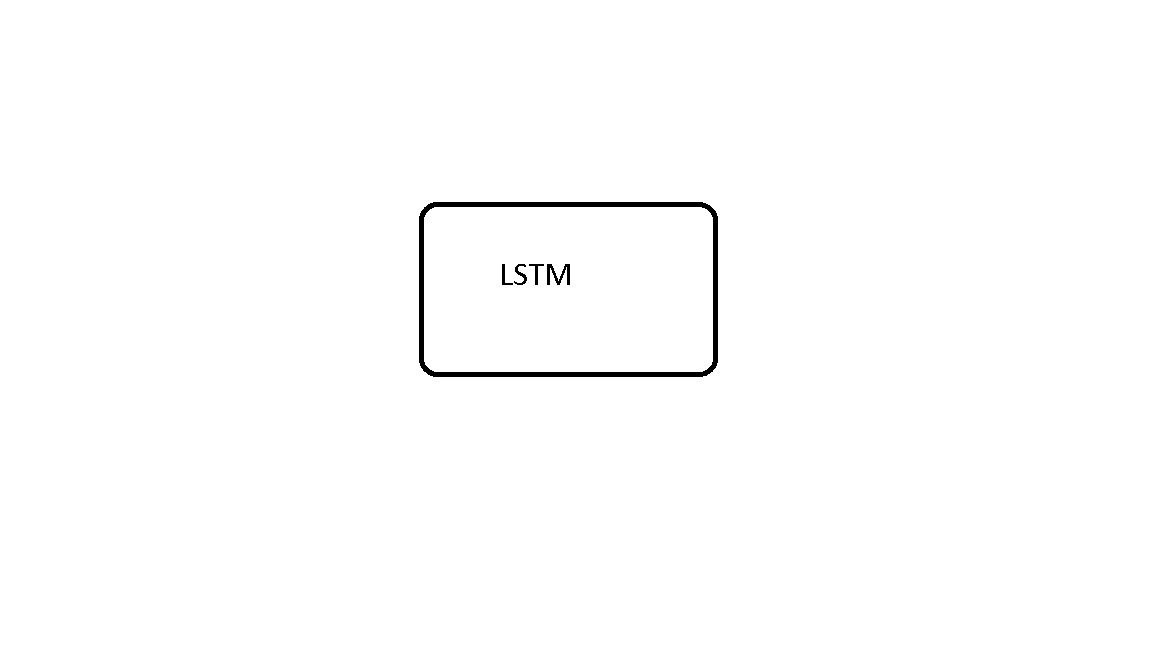
\includegraphics[width=0.25\textwidth]{imgs/LSTM-diagrama.jpg}
    \label{fig:diagrama-LSTM}
    \caption{Diagrama basico red LSTM}
    \end{figure}
Este tipo de redes son las mas utilizadas actualmente para realizar reconocimiento de 
caracteres, pero cuentan con la desventaja de requerir mayor poder de computo, por la necesidad
almacenar y anidar datos anteriores.

La otra alternativa que se utiliza es la de Redes Neuronales del tipo convulucional, que mediante 
el uso de convoluciones entre los pixeles de la imagen y una serie de matrices establecidas
extrae caracteristicas utilizadas para comparar la imagen con una lista de valores posibles,
dando por resultado el caracter que mas similitud tenga con el set de comparacion.
\begin{figure}[h]
    \centering
    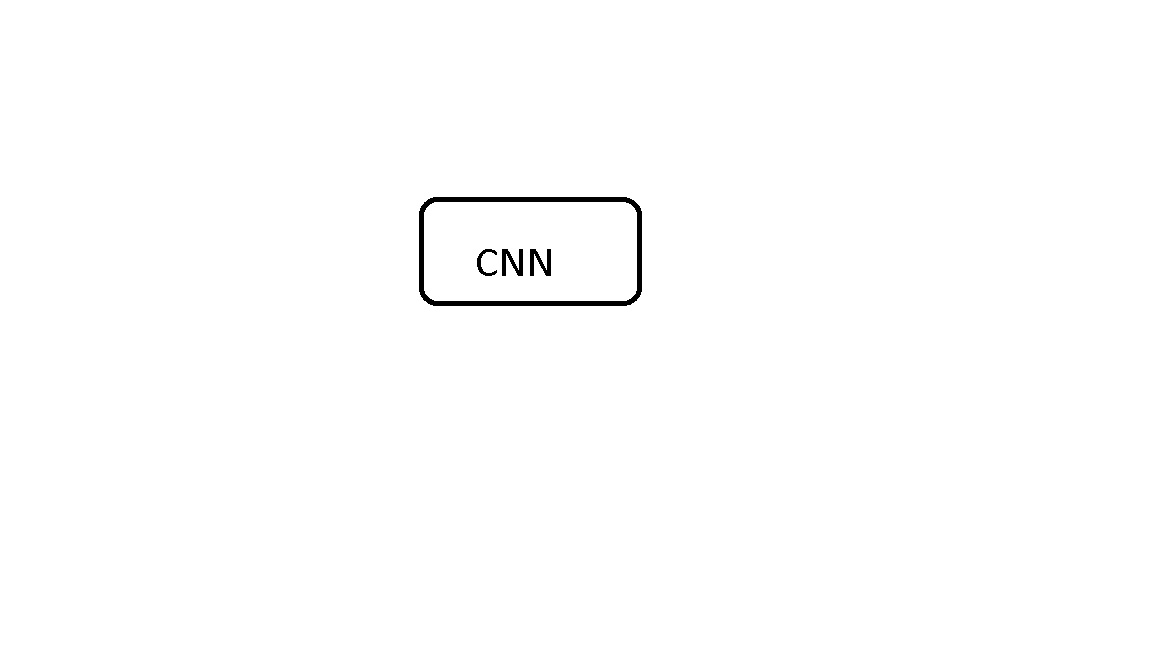
\includegraphics[width=0.25\textwidth]{imgs/CNN-diagrama.jpg}
    \label{fig:diagrama-CNN}
    \caption{Diagrama basico red CNN}
    \end{figure}

Al no requerir almacenar informacion ni trabajar de forma recursiva, la implementacion
de este tipo de redes pueden ser implementadas en equipos con un hardware de menor potencia,menor tamaño y 
por consiguiente menor costo.
\section{Marco teórico}

\section{Requerimientos necesarios de la red}

\section{Implementación del algoritmo en Python 3}
